\documentclass[a4paper,12pt]{scrartcl}

%Wir arbeiten mit PDF-Latex.
%Bei Texmaker unter Werkzeuge > PDFLaTeX (F6)

\usepackage[utf8x]{inputenc}

%Für deutsche Schriften:
%\usepackage[ngerman]{babel}
%\usepackage{sistyle}
%\SIstyle{German}
%\usepackage{icomma} % Komma als Dezimaltrenner (im Mathe Modus)
		    % Standardmäßig läßt LaTeX im Mathe Modus immer etwas 
		    % Platz nach einem Komma, für 3,45 etc. ist das falsch.
		    % Mit icomma gilt:
		    % Wenn auf das Komma ein Leerzeichen folgt, soll auch
		    % eins kommen, wenn nicht, schreibe es als Operator:
		    % z.B. $f(x, y) = 3,45$

%Für englische Schriften:
\usepackage[english]{babel}
\usepackage{sistyle}


\usepackage[top = 2cm, left = 2.5cm, right = 2cm, bottom = 2.5cm]{geometry}

\usepackage{amsmath}
\usepackage{amssymb}
\usepackage{array}

\usepackage{cite} %Für Zitate und Quellen
\usepackage{url}
\urlstyle{tt}

%\usepackage{longtable} % mehrseitige Tabellen
%\usepackage{multirow} %Zusammenfassen von Spalten/Zeilen



\usepackage{subfig} % Vereinen von Bildern in gesamte Figure

%Schönere Unterschriften für Bilder und Tabellen
%Setze captions mit Kommas und Beschriftungen
\DeclareCaptionLabelFormat{mycaption}{#1 #2}
\DeclareCaptionLabelSeparator{comma}{, }
\captionsetup{font=small,labelfont=bf,labelformat=mycaption,labelsep=comma}
\setcapindent{0pt} % Zeileneinzug ab zweiter Zeile

\newcommand{\mycaption}[2]{\caption[~#1]{\textbf{#1:} #2}}

\usepackage{textcomp} % Sonderzeichen
\usepackage{wrapfig}

\usepackage[svgnames]{xcolor} %Farben wie DarkBlue

%%
%%
%% Definitionen für schöne Links innerhalb des Dokuments
  %%% graphicx: support for graphics
  \usepackage[pdftex]{graphicx}


  \pdfcompresslevel=9

  %%% hyperref (hyperlinks in PDF): for more options or more detailed
  %%%          explanations, see the documentation of the hyperref-package
  \usepackage[%
    %%% general options
    pdftex=true,      %% sets up hyperref for use with the pdftex program
    %plainpages=false, %% set it to false, if pdflatex complains: ``destination with same identifier already exists''
    %
    pdfstartview={XYZ 0 0 1.0} , %% Startet das PDF mit 100% Zoom, also Originalgroesse
    %%% extension options
    backref,      %% adds a backlink text to the end of each item in the bibliography
    pagebackref=false, %% if true, creates backward references as a list of page numbers in the bibliography
    colorlinks=true,   %% turn on colored links (true is better for on-screen reading, false is better for printout versions)
    linkcolor=DarkBlue,		%% Aendern der Linkfarbe
    urlcolor=DarkBlue,		%% Aendern der Url-Linkfarbe und andere serioese Farben
    anchorcolor = black,
    citecolor = DarkGreen,
    filecolor = black,
    urlcolor = DarkBlue,
    breaklinks=false,
    %
    %%% PDF-specific display options
    bookmarks=true,          %% if true, generate PDF bookmarks (requires two passes of pdflatex)
    bookmarksopen=true,     %% if true, show all PDF bookmarks expanded
    bookmarksnumbered=false, %% if true, add the section numbers to the bookmarks
    %pdfstartpage={1},        %% determines, on which page the PDF file is opened
    %pdfpagemode=None         %% None, UseOutlines (=show bookmarks), UseThumbs (show thumbnails), FullScreen
  ]{hyperref}
  %%% provide all graphics (also) in this format, so you don't have
  %%% to add the file extensions to the \includegraphics-command
  %%% and/or you don't have to distinguish between generating
  %%% dvi/ps (through latex) and pdf (through pdflatex)
%  \DeclareGraphicsExtensions{.pdf}
%%
%%

%\newcommand{\kommentar}[1]{\marginpar{\textcolor{red}{#1}}}  % Kommentarkommando
%\newcommand{\fehler}[3]{\SI{(#1}{}\SI{\pm #2)}{#3}} % Fehlerkommando

%Ort für mögliche Bilddateien (Unterordner)
\graphicspath{{bilder/}{messwerte/}{auswertung/}}

%Neue Befehle
\newcommand{\hyref}[2]{\hyperref[#2]{#1~\ref{#2}}} %Schönerer link statt "link zu Bild \ref{im:bild}" -> "\hyref{link zu Bild}{im:bild}"

\newcommand{\mytilde}{\raisebox{-0.9ex}{\~{ }}}

% Tell latex how to break the program names
\hyphenation{Py-Corr-Fit Py-Scan-FCS}

\begin{document}



\vspace{-5em}
\begin{flushright}
	
\includegraphics[angle=0,width=35mm]{Images/TU_Logo_SW} \hspace{1em}
	\raisebox{-0.2em}{
\includegraphics[angle=0,width=40mm]{Images/SchwilleLogo} }
	
\includegraphics[angle=0,width=40mm]{Images/PyScanFCS_logo_dark.pdf} 
\end{flushright}
%\vspace{-3em}
\begin{center}\rule{\textwidth}{0.1ex}\par\end{center}
%\vspace{-4em}
%\begin{center}\rule{\textwidth}{0.1ex}\par\end{center}



\vspace{1em}

\noindent\begin{tabular}{ll}
\textbf{PyScanFCS - Data evaluation for perpendicular line scanning FCS}\\
\textit{Software Guide} \\
\\

 Paul Müller \\
 Biotechnology Center of the TU Dresden \\
 Date: \today 
 
\end{tabular}

\vspace{2em}

\tableofcontents


\newpage

\graphicspath{{Images/}}

\section{Introduction}

\subsection{Preface}
PyScanFCS processes photon arrival times recorded in perpendicular scanning FCS setups using the Flex02-01D/C correlator from \url{http://correlator.com}.
\\
\\
The PyScanFCS software provided is free software: you can redistribute it and/or modify it
under the terms of the GNU General Public License as published 
by the Free Software Foundation, either version 2 of the License, 
or (at your option) any later version.
\\
\\
An exemplary usage of PyScanFCS - delivering a proof of principle from calibration to data fitting - was shown in \cite{Mueller2014}.

\subsection{Prerequisites}
In order to use the PyScanFCS software, the following equipment is needed:

\subsubsection*{Hardware}
\begin{itemize}
\item A confocal laser scanning microscope (CLSM). For single-color one-focus SFCS, the CLSM should be capable of continuously scanning along a single line. For more sophisticated measurements, features like ``Multitrack mode'' for dual-color measurements and frame scanning for two-focus SFCS are required (LSM510, Zeiss, Germany).

\item One or two avalanche photo diodes (APD) for single or dual color detection. In addition, matching filters and beam splitters. The detection channels are referred to as channels A and B throughout this documentation.

\item A photon stream recording device connected to the APDs. In the tested setup a Flex02-12D/B correlator from correlator.com\footnote{Note that for some reason the photon history recording mode does not work with the Flex02-01D/C correlator. Keep that in mind while troubleshooting your setup. When using a different device, the data has to be converted accordingly. The data format is described in \hyref{section}{sec:datformat}.} was used in photon history recording mode. The device creates two binary files A and B that contain the photon arrival times detected by the corresponding APDs.
\end{itemize}

\subsubsection*{Software}
PyScanFCS can be downloaded from \url{http://pyscanfcs.craban.de}.
\begin{itemize}
\item \textbf{Windows}
For Windows XP or Windows 7, stand-alone binary executables are available from the download page. 
\item \textbf{Linux}
There are executable binaries for widely used distributions (e.g. Ubuntu).
\item \textbf{Sources}
The program is written in python 2.7. On any operating system, PyScanFCS can be run from source. In general, the following packages need to be available:
\texttt{\\
cython ($\geq$ 0.1.6)\\
python-matplotlib ($\geq$ 1.0.1) \\
python-multipletau ($\geq$ 0.1.4) \\
python-numpy ($\geq$ 1.6.2) \\
python-pyfits \\
python-scipy ($\geq$ 0.10.1) \\
python-wxtools \\
python-wxgtk2.8-dbg \\
}
\\
There are two ways to make PyScanFCS run from source.\\
\textbf{Recommended way:} Install via pip
\texttt{ pip install pyscanfcs}
and run the package directly
\texttt{python -m pyscanfcs}.
\\
\textbf{Second way:}
Obtain the source directly from GitHub (\url{https://github.com/paulmueller/PyScanFCS}).


\paragraph*{Cython}
PyScanFCS needs Cython to perform some CPU intensive operations. Before running PyScanFCS from source, a C compiler needs to be installed (\url{http://docs.cython.org/src/quickstart/install.html}).
\begin{itemize}
\item[ ] \textbf{Windows}. The common MinGW compiler can be used. Instructions on how to install MinGW can be found in the Cython documentation: \url{http://docs.cython.org/src/tutorial/appendix.html}. On machines running Windows 7 x64 with the x64 version of python, the Microsoft Windows SDK for Windows 7 and .NET Framework 3.5 SP1 must be used: \\
\url{http://wiki.cython.org/64BitCythonExtensionsOnWindows}.

\item[ ] \textbf{Ubuntu}. The following packages need to be installed:
\\
\texttt{build-essential\\
python-dev} 
\item[ ] \textbf{MacOS}. This should work with Apple's XCode, available from \url{http://developer.apple.com}. It has not been tested.
\end{itemize}
Cython can be obtained from \url{http://www.cython.org/}. After unpacking of the archive, Cython is installed by executing \texttt{python setup.py install} within the unpacked directory\footnote{Cython can also be installed via PyPI (\url{http://pypi.python.org/pypi}).}.

For older version of Ubuntu, some of the above package versions are not listed in the package repository. To enable the use of PyScanFCS on those systems, the following packages need to be installed separately:

\begin{itemize}
\item[ ] \textbf{matplotlib}. The tukss-ppa includes version 1.0.1. After adding the repository (\texttt{apt-add-repository ppa:tukss/ppa}), matplotlib can be installed as usual.
\item[ ] \textbf{numpy}. The package from a later version of Ubuntu can be installed: \url{https://launchpad.net/ubuntu/+source/python-numpy/}
\item[ ] \textbf{scipy}. The package from a later version of Ubuntu can be installed: \url{https://launchpad.net/ubuntu/+source/python-scipy/}
\end{itemize}

\end{itemize}

Correlation curves created by PyScanFCS can be processed using \texttt{PyCorrFit}\footnote{\url{http://pycorrfit.craban.de}}.

\section{Data acquisition modes}
\begin{figure}[t]
\centering
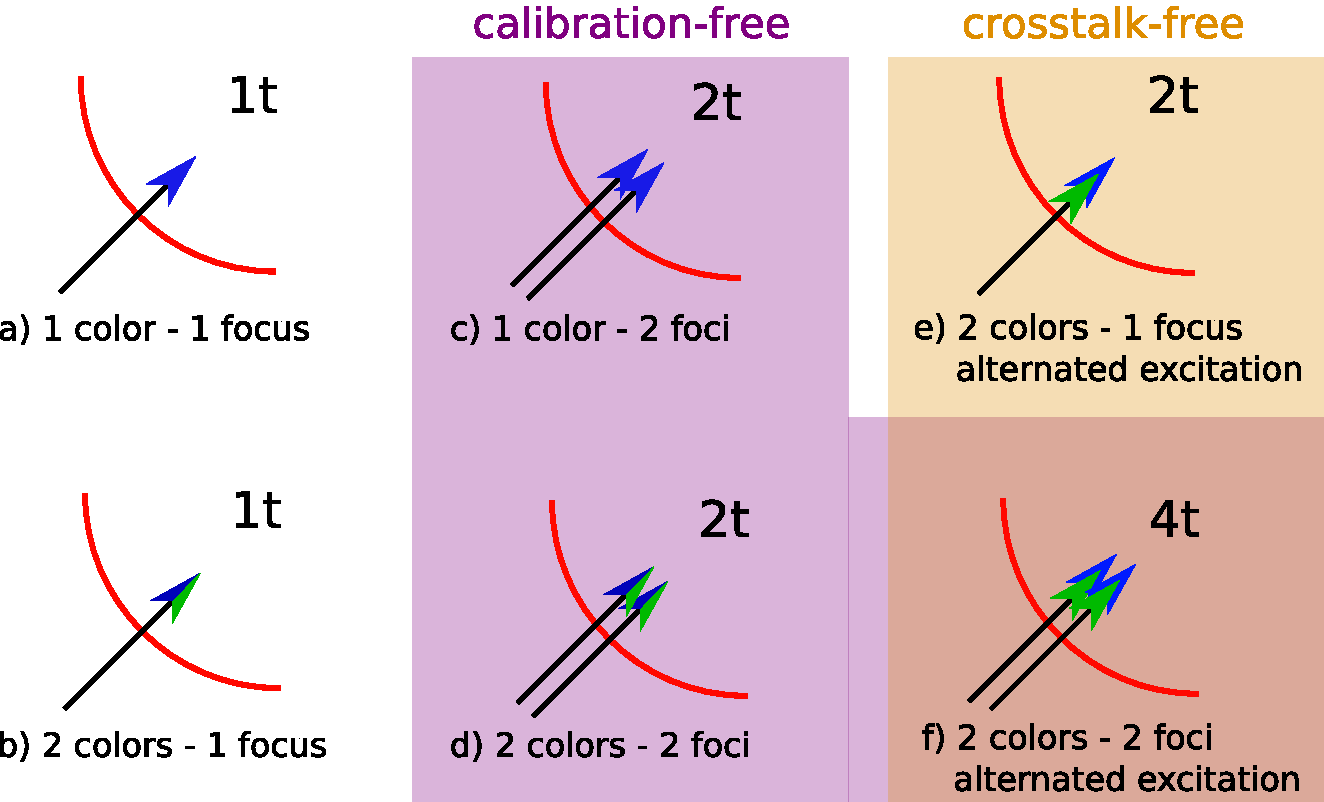
\includegraphics[width=0.8\linewidth]{SFCSmodi.pdf}
 \mycaption{acquisition modes in PyScanFCS}{The six figures \textbf{a-f} show possible scenarios for scan path and excitation settings. The alignment of the scan paths (black) is shown for membrane of a giant unilamellar vesicle (red). The arrow tips define the different colors used for each scan (blue excitation, green excitation, or both at the same time). Multiple arrow tips indicate the sequential scanning of one line with two colors. The time necessary to perform a complete scan in each scanning mode is shown respective to ``one color – one focus'' on the top right corner of each figure.\label{fig:scanmodi}}
\end{figure}
In order to achieve all possible measurement modes depicted in \hyref{figure}{fig:scanmodi}, the CLSM needs to be set up properly. The scan paths should be checked for straightness e.g. by bleaching a layer of eGFP\footnote{Often, hysteresis effects occur during high speed scanning and scan paths are not straight. Switching to slower bidirectional scanning or setting up a ``multitrack mode'' might solve these problems.}. In 2fSFCS, the distance between the lines can be determined in a similar fashion. For each measurement, it is vital to record approximate scanning time and channel assignment. PyScanFCS attempts to find the correct scanning cycle, but manual intervention will be necessary in case of a failure\footnote{In some cases, the microscope software (AIM, Zeiss) might also calculate a wrong scan cycle time.}.
\begin{figure}[]
\centering
% 2012-08-27-SFCS_DiO-DOPC-GUVs --> GUV5b
\subfloat[SFCS: GUV scan path][GUV scan path in SFCS]
{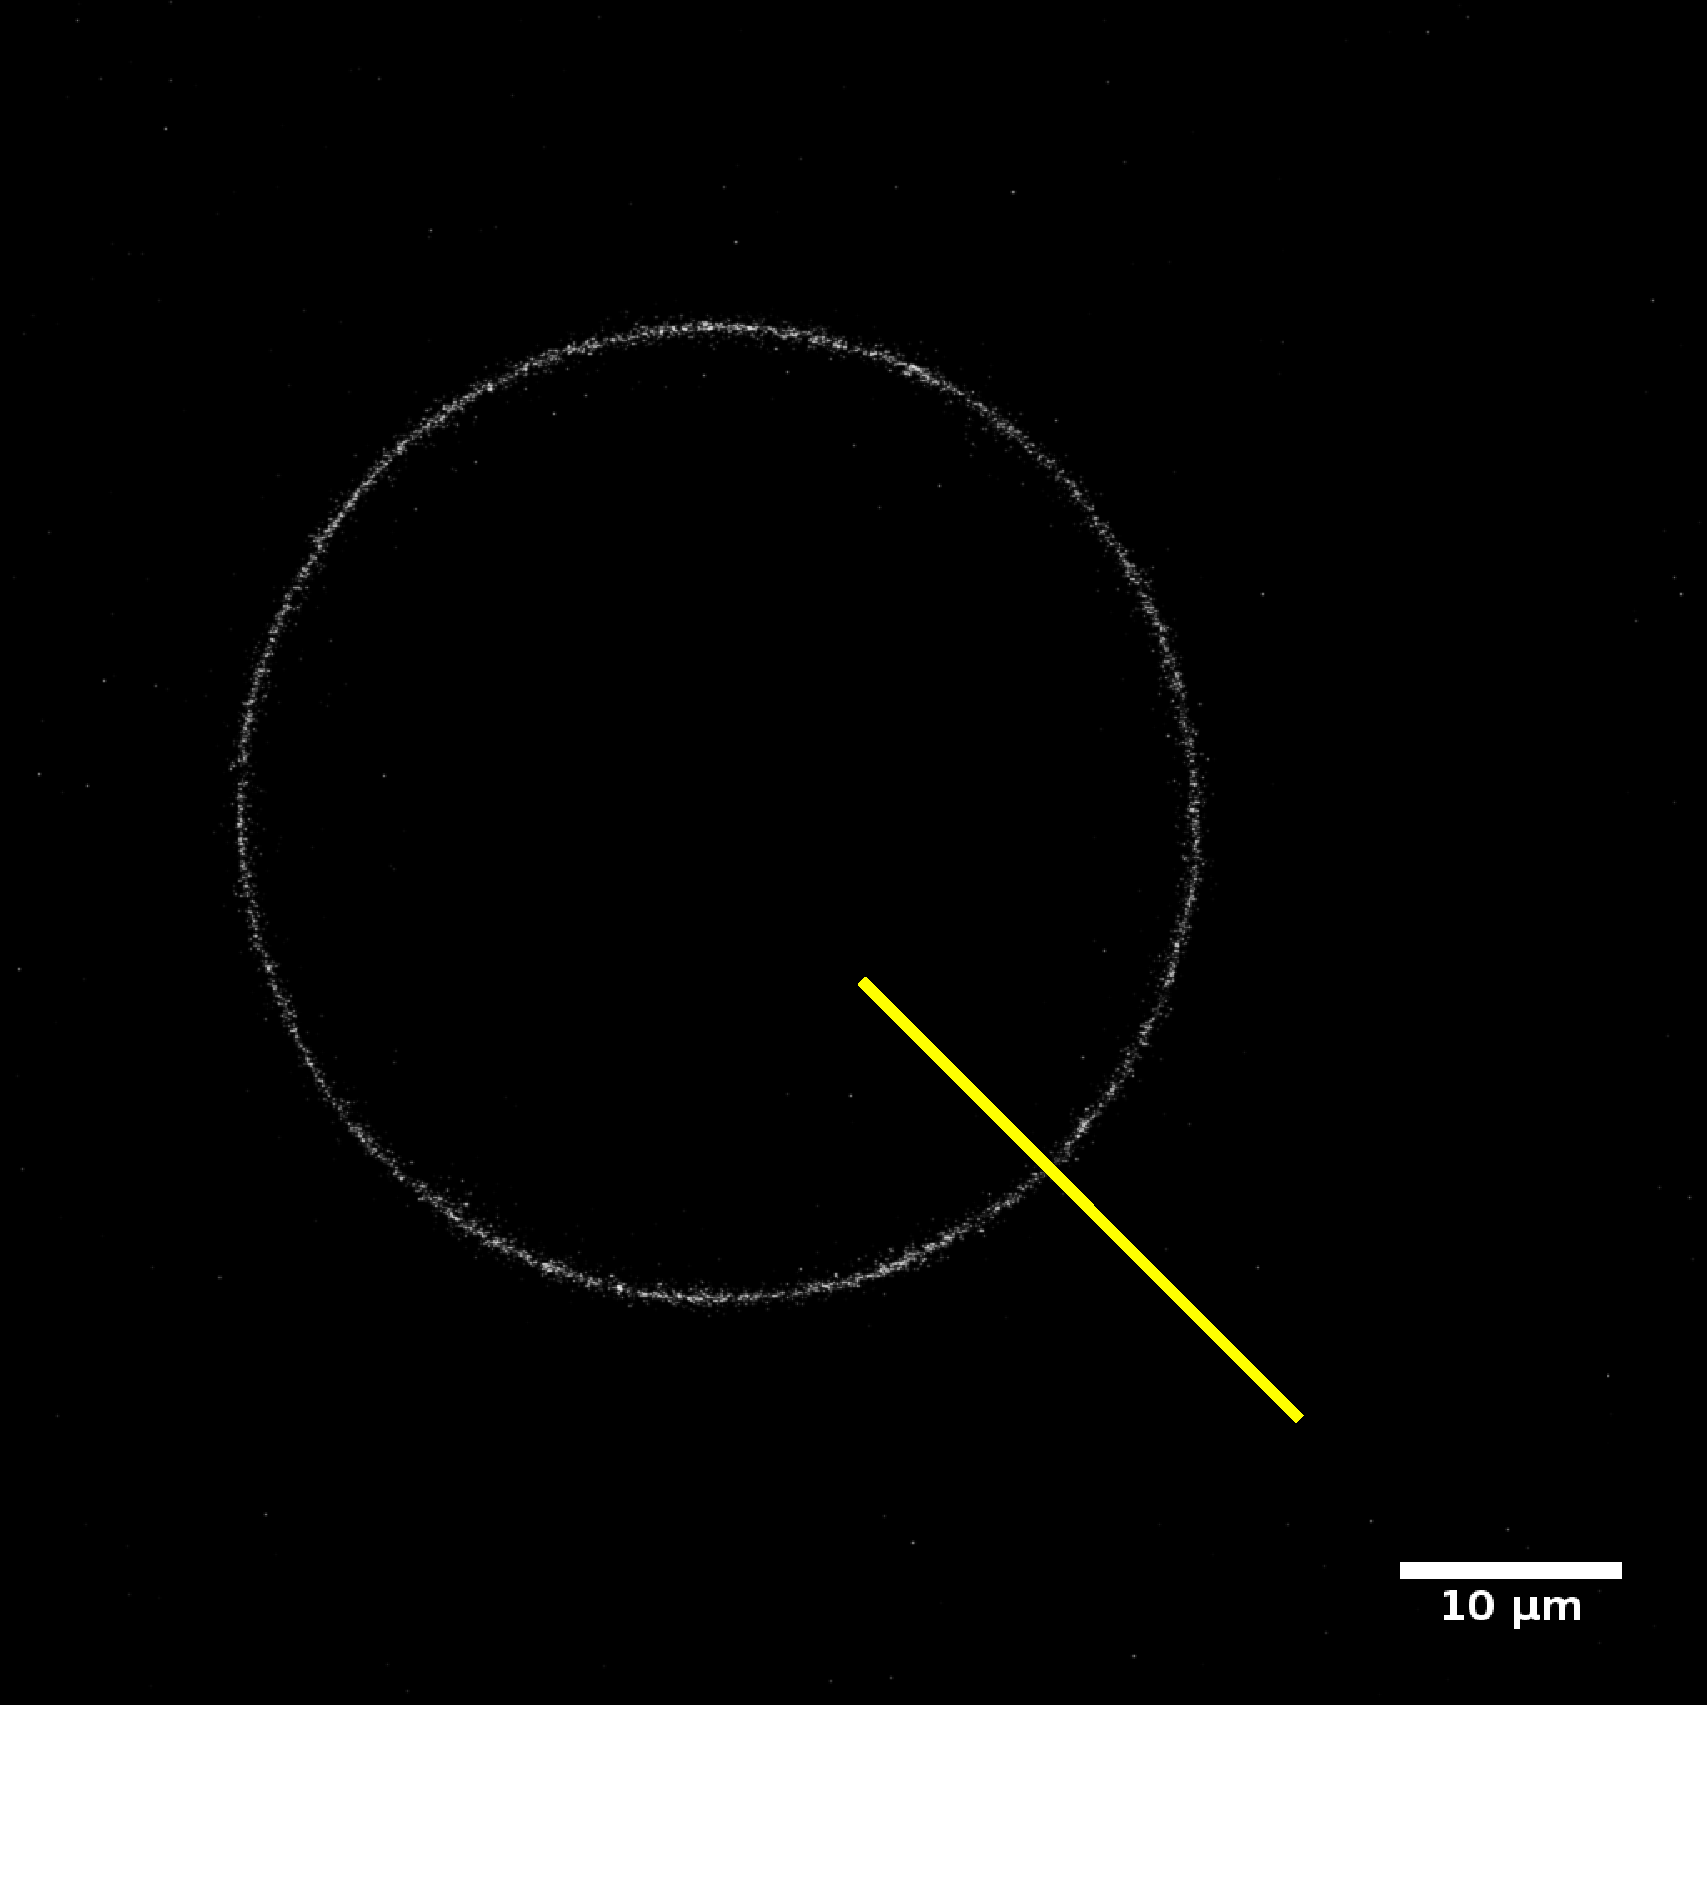
\includegraphics[width=0.34\linewidth]{GUV.pdf}} \qquad
\subfloat[SFCS: Kymograph][Kymograph produced by PyScanFCS]
{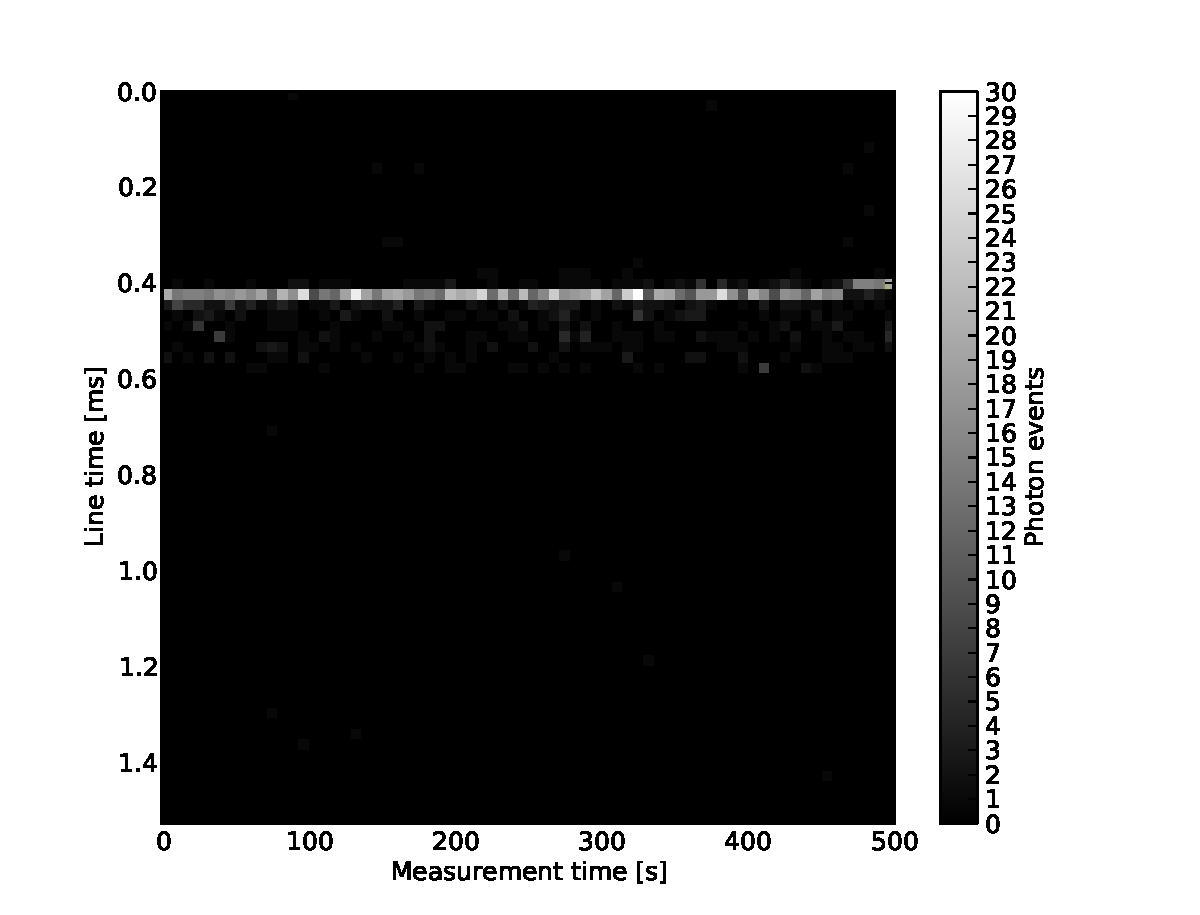
\includegraphics[width=0.55\linewidth]{1color1focus.pdf}} 
 \mycaption{1 focus 1 color measurement with PyScanFCS}{ \label{fig:1c1f_example} Example of a GUV scanned using one focus and one laser line. \textbf{a)} The equator of a GUV with the scan path (yellow). \textbf{b)} A kymograph generated by PyScanFCS. The scan cycle time is \SI{1.527}{ms} (vertical) and the measurement time is \SI{500}{s} (horizontal). Each scan cycle is binned into 70 bins. Note that the resolution in direction of the measurement time is adapted to the scan cycle resolution. Also note the step at the end of the measurement. Such a step can be the result of a movement of the GUV during the measurement. This part needs to be excluded from the trace before calculating the correlation function.}
\end{figure}
This section describes the acquisition modes that PyScanFCS supports. Correlation functions are labeled according to \hyref{figure}{fig:example_kymograph}. \hyref{Figure}{fig:scanmodi} shows advantages and disadvantages in terms of time resolution, calibration and crosstalk.
\paragraph{a) one color - one focus}
One spot of the membrane is scanned continuously using one laser line. The signal is detected using one APD and PyCanFCS can be used to calculate one autocorrelation curve ($AC_{A1}$).
\paragraph{b) two colors - one focus}
The setup is the same as in (a), except that two laser lines are used and the signal is detected by two APDs. This mode can be applied for multiple dye studies. There are four possible correlations: $AC_{A1}$, $AC_{B1}$, $CC_{A1B1}$, $CC_{B1A1}$

\paragraph{c) one color - two foci}
The CLSM is set up to perform a line scan along two lines with a distance $d$ apart. For detection, only one APD is required. The distance $d$ needs to be determined beforehand. In addition to two autocorrelations, two cross correlation curves are obtained. The cross correlation curves contain information about the shape and size of the focus traversing the membrane. Thus, no calibration measurement with a reference dye is necessary to determine extents of the scanning focus.
Possible correlations: $AC_{A1}$, $AC_{A2}$, $CC_{A1A2}$, $CC_{A2A1}$


\paragraph{d) two colors - two foci}
Like (b), this is a dual-color extension. Two laser lines are used for scanning and two APDs are used for detection.\\
Possible autocorrelations: 4\\
Possible cross-correlations: 12

\paragraph{e,f) dual color with alternating excitation}
To avoid cross-talk between the two color channels, as it likely happens in the \textit{b) two colors - one focus} or \textit{d) two colors - two foci}  modes, the CLSM can be setup to sequentially scan the membrane with two laser lines. This way, only one laser line is used to excite the sample at a time and the fluorescence of two dyes can be separated, effectively circumventing crosstalk. The scan cycle time  doubles when using alternating excitation and hence the binning time is twice as long. This effectively results in ``loosing'' data points\footnote{For the multiple-$\tau$ algorithm used, exactly $m/2$ points are lost, where $m$ is the number of points of the correlation curve that are calculated by the multiple-$\tau$ algorithm before the intensity trace is binned for the first time.}  at the beginning of the correlation curve, which decreases the time resolution.\\
Possible correlations (1 focus): $AC_{A1}$, $AC_{B2}$\\
Possible correlations (2 foci): $AC_{A1}$, $AC_{B2}$, $CC_{A1B2}$, $CC_{B2A1}$

\begin{figure}[h]
\centering
\subfloat[][A: Red channel]
{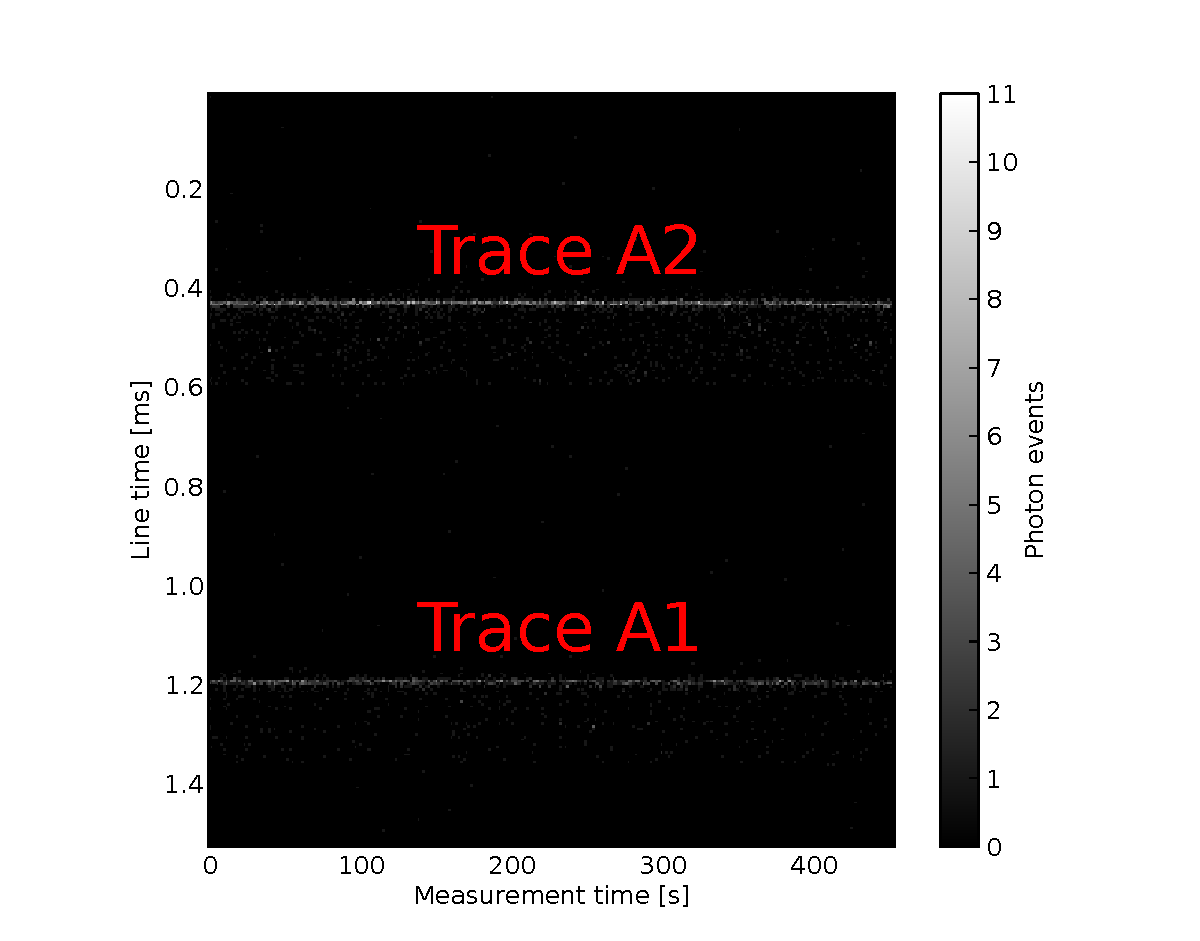
\includegraphics[width=0.45\linewidth]{alexA.pdf}} \qquad
\subfloat[][B: Green channel]
{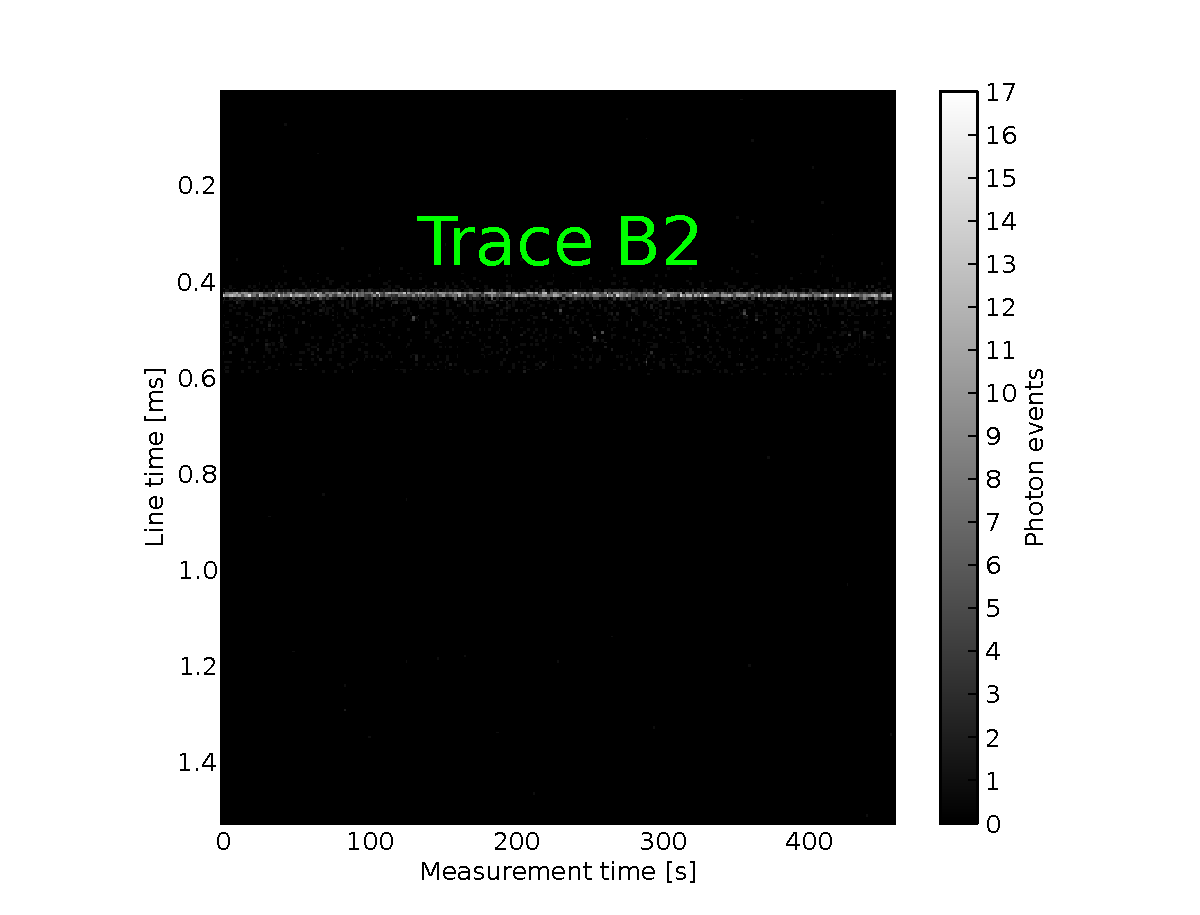
\includegraphics[width=0.45\linewidth]{alexB.pdf}} 
 \mycaption{alternating excitation with PyScanFCS}{ \label{fig:example_kymograph} The kymograph yields a scanning time for one line of \SI{1.527}{ms}. One can clearly see the trace A2, which originates from crosstalk from the green dye to the red channel or from the red dye being excited by the green laser. There is no crosstalk from the red dye to the green channel, which in this case helps identify the traces.}
\end{figure}

\section{Working with PyScanFCS}
\subsection{Data file formats}
\begin{itemize}

\item \textbf{\mytilde .csv files} each contain a correlation curve. Further information is available in the \texttt{PyCorrFit} documentation (\url{http://pycorrfit.craban.de}).

\label{sec:datformat}
\item \textbf{\mytilde .dat files} are created by the software \texttt{Photon.exe} that ships with the correlators from correlator.com. The format stores the photon arrival time differences between two photon events. Data format is as follows\footnote{Note, that Windows uses the little endian byte order. This might lead to problems when using PowerPC.}:
	\begin{itemize}
	\item The value of the first byte (uint8) identifies the format of the file: 8, 16, or 32 bit.
	\item The value of the second byte (uint8) identifies the system clock, usually \SI{60}{MHz}.
	\item The rest of the file contains the times between two photon arrivals. The time unit is 1/(system clock) (here \SI{16.\overline{66}}{ns}).
	\item 8 bit format is not supported.
	\item 16 bit format. Each word (2 bytes, uint16) represents a photon event. For low intensities, values of \texttt{0xFFFF} may occur. In this case, the following four bytes (uint32) represent a photon event.
	\item 32 bit format. Each dword (4 bytes, uint32) represents a photon event. 32 bit files can be created from 16 bit files using \texttt{Photon.exe}. PyScanFCS saves \mytilde .dat files in this format.
 	\end{itemize}
\item \textbf{\mytilde .fits files} - The \textbf{f}lexible \textbf{i}mage \textbf{t}ransport \textbf{s}ystem is used by PyScanFCS to save already binned \mytilde .dat files. Those files contain additional fits-keys:
	\begin{itemize}
	\item \texttt{SysClck} - system clock in MHz
	\item \texttt{Total} - total measurement time in system clock ticks
	\item \texttt{Tcycle} - acquired scan cycle time in system clock ticks
	\item \texttt{Tbin} - binning of the photon events in system clock ticks
	\item \texttt{Binshift} - bins added to beginning of the entire 2D data array before plotting

	\end{itemize}
	Because these files can become quite large, it is not recommended to store the data in this file format. Also, information is lost due to the binning. It is possible to save a \mytilde .fits file with only a few photon events binned (small file size), which contains the correct plotting parameters (cycle time, bin shift). This file can later be opened prior to opening the corresponding \mytilde .dat file. This way, e.g. the scan cycle time does not have to be found again.

\item \textbf{\mytilde .int files} are created during binning. They are straight 16 bit files that contain binned events from a \mytilde .dat file.

\item \textbf{\mytilde .txt files} are generated optionally, if the user wants to save the generated traces. The file contains photon numbers, separated by a new line. The binning time, as well as the corresponding intensities can be calculated from parameters given in the file.

\item \textbf{\mytilde .zip files} are bundles of correlation curves ( - stored as \mytilde .csv files). They can be imported for fitting by \texttt{PyCorrFit}. \mytilde .zip files are automatically stored in the working directory (location of \mytilde .dat or \mytilde .fits files).

\end{itemize}



\subsection{The user interface}
\begin{figure}[h]
\centering
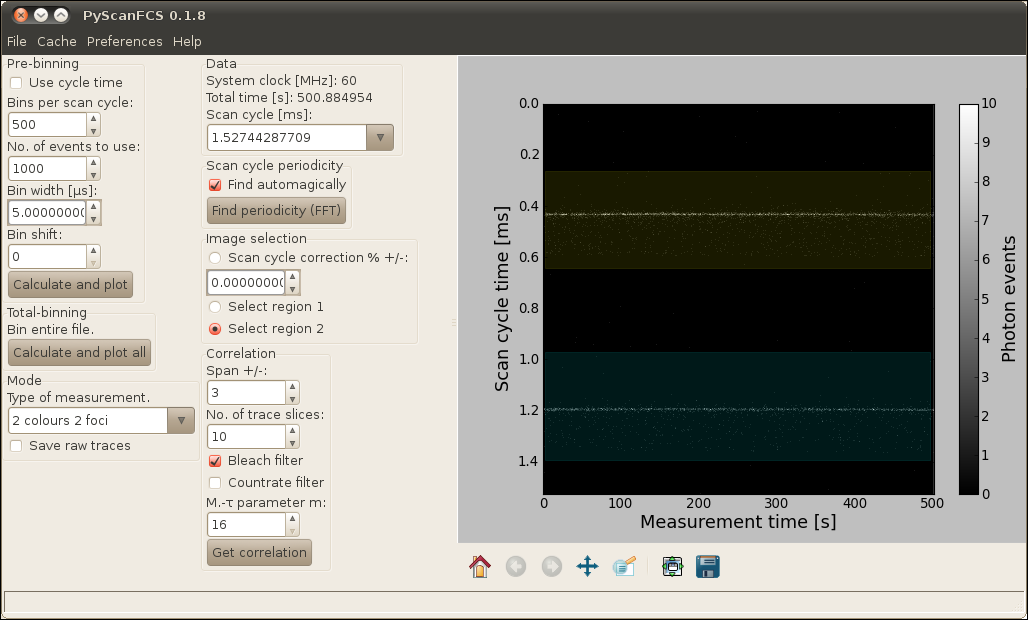
\includegraphics[width=0.95\linewidth]{PyScanFCS_Main.png}
 \mycaption{user interface}{The left panel displays all parameters. The right panel shows the kymograph of the measurement. \label{fig:SFCSMain}}
\end{figure}
\hyref{Figure}{fig:SFCSMain} shows the main user interface with the following content:
\begin{itemize}
\item The \textbf{menu bar} with standard operations, such as loading or saving a file. The \textbf{cache menu} is a convenience tool. It displays all previously binned \mytilde .dat files.

\item \textbf{Pre-binning}: This sets up all parameters that are used to bin a \mytilde .dat file:
	\begin{itemize}
	\item[-] the binning resolution of the scan cycles
	\item[-] the number of events from a \mytilde .dat file to process
	\item[-] the bin width of a scan cycle (not used if the scan cylce time is known)
	\item[-] a bin shift can be used to help selecting traces
	\end{itemize}
The bin shift parameter adds a number of empty bins to the beginning of the binned array. This will shift the vertical (scan cycle time) position of the visible trace.

\item \textbf{Total-binning}: Bin the entire file using the scan cycle time found.

\item \textbf{Mode}: Selects which mode to use. The modes are described above. Optionally save traces as \mytilde .txt files inside the working directory.

\item \textbf{Data}: Displays current file information and found scan cycle time. The scan cycle time may be doubled, quadrupled, halved or quartered. This may help, if the automagic algorithm did not find the correct scan cycle time.

\item  \textbf{Find line scan time}: Performs a fourier transform of the binned data\footnote{The user is advised to not use too many events. This might result in a system lock-up.}. If the check box is activated, the program will automatically find the correct maximum in fourier space and write back the corresponding scan cycle time. If the check box is not activated, a window will pop up for the user to define an interval where to search for a maximum. When a scan cycle time has been found, then the check box in \textbf{Pre-binning} will become active.

\item  \textbf{Image selection}: Selects which tool to apply to the binned image in the \textbf{kymograph}. This does not work, if any other tool (e.g. magnifier) from the kymograph toolbar is active.
	\begin{itemize}
	\item[-] scan cycle correction: This is used, if the scan cycle time found is not exactly correct (tilted lines in the kymograph). To correct the scan cylce time, the user draws a line along the trace in the kymograph. Afterwards, the kymograph can be recalculated using \textbf{Pre-Binning} or \textbf{Total-binning}.
	\item[-] Select region 1: Lets the user draw a rectangle around a trace that should be used for correlation. Region 1 is always displayed in yellow.
	\item[-] Select region 2: Depending on the \texttt{mode}, the user may select a second region for additional auto- and cross-correlation. Region 2 is always displayed in cyan.
	\item[-] Full measurement time: Maximizes the measurement time selection (horizontal in the kymograph) for the regions.
	\end{itemize}
	
\item \textbf{Correlation}: Calculates the traces and perform the multiple-$\tau$ algorithm according to the selected \textbf{mode}. 
	\begin{itemize}
	\item[-] Span: The trace is calculated from the maximum of each scanned line. This corrects for spacial fluctuations perpendicular to the surface of the probed membrane. If the binning is too fine, or the scan cycle time is not exactly correct, this number can be increased to include more neighboring bins for the calculation of the trace.
	\item[-] No. of trace slices: Sometimes, dirt contaminates the trace. The trace can be split and the correlation curves can be calculated separately from each slice. \texttt{PyCorrFit} is able to average over user selected curves, yielding cleaner statistics.
	\item[-] Bleach filter: Fits an exponential function to the selected trace and performs a bleaching correction according to \cite{Ries2009}. Note that this bleaching correction is only valid for an approximately linear decay in the fluorescence signal. The bleaching data is exported to the zip file that also contains the correlation data. They are named
	\begin{center}
	\texttt{PyScanFCS\_bleach\_profile\_TYPE\_RANDOM.csv}
	\end{center}
	where  \texttt{TYPE} is the type of the curve (e.g. \texttt{Region\_A1}) and \texttt{RANDOM} is just a random number.
	\item[-] Countrate filter: Approximates the count rate of the fluorescence signal from the membrane. Because the laser focus is \textit{scanned} through the membrane, the average signal from the measurement does not equal the actual count rate within the membrane. The algorithm fits a Gaussian to the average intensity profile and uses the standard deviation to calculate the residence time of the focus inside the membrane.	This residence time is then used to calculate the approximate count rate.
	\item[-] M.-$\tau$ parameter m: This is a parameter of the multiple-$\tau$ algorithm. $m$ is the number of points of the correlation curve that are calculated by the multiple-$\tau$ algorithm in the first loop. Afterwards, the intensity trace is binned by combining two neighboring bins. Then, sequentially $m/2$ data points are calculated after each binning of the trace. A thorough description is given in \cite{Wohland2001}. $m=16$ is a good measure.

	\end{itemize}
\item The \textbf{kymograph plot} shows the binned \mytilde .dat files. The Pixel resolution in the direction of measurement time is adjusted to match the resolution of the scan cycle time (bins per scan cycle). This is implemented by slicing the array and showing only a few slices in measurement time ``direction''. So far, no disadvantages compared to averaging have been observed. The plotting area contains a useful toolbar.
\end{itemize}




\section*{Acknowledgements}
\addcontentsline{toc}{section}{Acknowledgements}
I thank Eugene Petrov and Fabian Heinemann (MPI Biochem, Martinsried, Germany) for discussions on the implementation of the multiple-$\tau$ algorithm. I thank André Scholich (TU Dresden, Germany) for initial proof reading of the manuscript. The idea of a kymograph and the Fourier analysis method are adopted from a Matlab script written on the same issue by Jonas Ries.


%%%%%%%%%%%%%%%%%%%%%%%%%%%%%%%%%%%%%%%%%%%%%%%%%%%%%%%%%%%%%%%%%%%%%%%%%%%%%
% Literaturverzeichnis

\pagestyle{plain}             % nur Nummerierung in der Fußzeile

\bibliographystyle{unsrt}  % Zitierstil: alphadin = [Nam88] apt-get install bibtex-extras
\bibliography{Bibliography}      % BibTeX-Datei name.bib ohne .bib hier einfgen
%\nocite{*}                    % Listet alle Eintrge der Datei auf, wenn aktiv


\end{document}
